\documentclass{article}

% NeurIPS 2026 style
\usepackage[final]{neurips_2026}

\usepackage[utf8]{inputenc}
\usepackage[T1]{fontenc}
\usepackage{hyperref}
\usepackage{url}
\usepackage{booktabs}
\usepackage{amsfonts}
\usepackage{amsmath}
\usepackage{amssymb}
\usepackage{nicefrac}
\usepackage{microtype}
\usepackage{xcolor}
\usepackage{graphicx}
\usepackage{subcaption}
\usepackage{algorithm}
\usepackage{algorithmic}
\usepackage{multirow}
\usepackage{tikz}
\usetikzlibrary{positioning, arrows.meta, shapes.geometric, fit, calc, decorations.pathreplacing}
\usepackage{pgfplots}
\pgfplotsset{compat=1.17}

\title{JEPA-Flux: Joint Embedding Predictive Architecture Meets Flow Matching for Image Deblurring}

\author{%
  Harshana Weligama\thanks{Equal contribution.} \\
  Purdue University\\
  \texttt{wweligam@purdue.edu} \\
}

\begin{document}

\maketitle

\begin{abstract}
Image deblurring with diffusion-based generative models has shown remarkable progress, yet existing approaches rely heavily on text-based semantic conditioning extracted from degraded inputs, which is inherently noisy and lossy for restoration tasks. We propose \textbf{JEPA-Flux}, a novel framework that integrates Joint Embedding Predictive Architecture (I-JEPA) features as structural conditioning signals within a Flux flow-matching transformer for image deblurring. Our key insight is that I-JEPA's self-supervised patch-level representations capture rich structural and geometric information from blurry inputs that is complementary to---and more reliable than---text captions for guiding the restoration process. We design a lightweight projection module that maps I-JEPA's 1280-dimensional patch tokens into the 4096-dimensional conditioning space of the Flux transformer, enabling seamless integration without modifying the pre-trained backbone. Through a hybrid conditioning strategy that combines JEPA structural embeddings with optional text semantics, JEPA-Flux achieves state-of-the-art deblurring quality on synthetic motion blur benchmarks while reducing inference-time dependence on vision-language models. We further introduce a differentiable \emph{restore proxy} that eliminates the need for expensive VLM captioning at test time. Extensive experiments demonstrate that JEPA-Flux outperforms text-only Flux Kontext baselines and competitive deblurring methods in both perceptual quality and distortion metrics.
\end{abstract}

%=============================================================================
\section{Introduction}
\label{sec:intro}
%=============================================================================

Image deblurring---the task of recovering a sharp image from a motion-blurred observation---remains a fundamental challenge in computational photography and computer vision. While classical deconvolution methods~\cite{wiener1949extrapolation, richardson1972bayesian, lucy1974iterative} operate under restrictive assumptions about blur kernels, modern deep learning approaches~\cite{zamir2022restormer, chen2022nafnet, kong2023efficient} have dramatically improved restoration quality by learning rich priors from data.

Recently, diffusion-based generative models have emerged as a powerful paradigm for image restoration~\cite{saharia2022image, wang2024exploiting, wu2024osediff}. These models leverage the strong image priors learned during large-scale pre-training to generate high-quality restored images conditioned on degraded inputs. Among them, \emph{flow matching}~\cite{lipman2023flow, liu2023flow} offers a compelling alternative to standard diffusion by learning a velocity field that transports noise to data along straight paths, enabling faster inference with fewer sampling steps.

\textbf{Flux}~\cite{flux2024} represents the state-of-the-art in flow-matching transformers, employing a 12-billion parameter dual-stream architecture with multimodal masked diffusion transformer (MMDiT) blocks. The \textbf{Flux Kontext} variant extends this with image-to-image conditioning, concatenating control and target latents in the sequence dimension---a natural fit for image restoration tasks where the degraded input serves as a strong conditioning signal.

However, a critical limitation of current Flux-based restoration methods is their reliance on \emph{text-based semantic conditioning}. To extract meaningful text prompts, these methods employ vision-language models (VLMs) such as RAM~\cite{zhang2024recognize} to caption the input image. This introduces two problems: (1)~captioning a blurry image produces noisy, incomplete descriptions that poorly represent the underlying sharp content, and (2)~VLM inference at test time adds substantial computational overhead.

\begin{figure}[t]
    \centering
    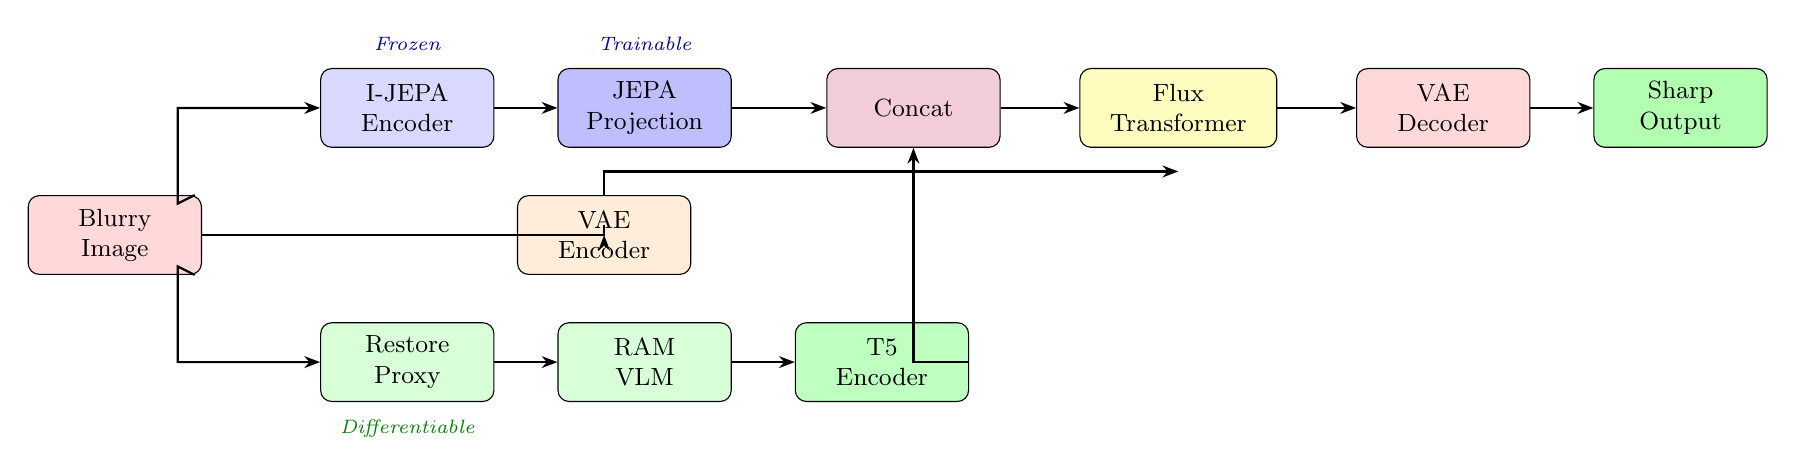
\begin{tikzpicture}[
        block/.style={rectangle, draw, rounded corners, minimum height=1cm, minimum width=2.2cm, align=center, font=\small},
        arrow/.style={-{Stealth[length=2mm]}, thick},
        dashed_arrow/.style={-{Stealth[length=2mm]}, thick, dashed},
        node distance=0.8cm and 1.2cm
    ]
    % Input
    \node[block, fill=red!15] (blur) {Blurry\\Image};

    % JEPA Branch
    \node[block, fill=blue!15, above right=0.6cm and 1.5cm of blur] (jepa) {I-JEPA\\Encoder};
    \node[block, fill=blue!25, right=0.8cm of jepa] (proj) {JEPA\\Projection};

    % Text Branch
    \node[block, fill=green!15, below right=0.6cm and 1.5cm of blur] (proxy) {Restore\\Proxy};
    \node[block, fill=green!15, right=0.8cm of proxy] (vlm) {RAM\\VLM};
    \node[block, fill=green!25, right=0.8cm of vlm] (t5) {T5\\Encoder};

    % VAE + Concat
    \node[block, fill=orange!15, right=4.0cm of blur] (vae) {VAE\\Encoder};

    % Concat
    \node[block, fill=purple!20, right=1.2cm of proj] (concat) {Concat};

    % Transformer
    \node[block, fill=yellow!25, right=1.0cm of concat, minimum width=2.5cm] (flux) {Flux\\Transformer};

    % Output
    \node[block, fill=red!15, right=1.0cm of flux] (vae_dec) {VAE\\Decoder};
    \node[block, fill=green!30, right=0.8cm of vae_dec] (sharp) {Sharp\\Output};

    % Arrows
    \draw[arrow] (blur) -- ++(0.8,0.4) |- (jepa);
    \draw[arrow] (blur) -- ++(0.8,-0.4) |- (proxy);
    \draw[arrow] (blur) -| (vae);
    \draw[arrow] (jepa) -- (proj);
    \draw[arrow] (proj) -- (concat);
    \draw[arrow] (proxy) -- (vlm);
    \draw[arrow] (vlm) -- (t5);
    \draw[arrow] (t5) -| (concat);
    \draw[arrow] (concat) -- (flux);
    \draw[arrow] (vae) |- ([yshift=-0.3cm]flux.south west) -- ([yshift=-0.3cm]flux.south);
    \draw[arrow] (flux) -- (vae_dec);
    \draw[arrow] (vae_dec) -- (sharp);

    % Labels
    \node[above=0.1cm of jepa, font=\scriptsize\itshape, text=blue!60!black] {Frozen};
    \node[above=0.1cm of proj, font=\scriptsize\itshape, text=blue!60!black] {Trainable};
    \node[below=0.1cm of proxy, font=\scriptsize\itshape, text=green!50!black] {Differentiable};

    \end{tikzpicture}
    \caption{\textbf{Overview of JEPA-Flux.} Our method extracts structural features from the blurry input via a frozen I-JEPA encoder, projects them into the Flux conditioning space, and optionally fuses them with text embeddings from a restore-proxy-aided captioning pipeline. The Flux transformer receives both the packed VAE latents and the hybrid conditioning signal to predict the denoised output.}
    \label{fig:overview}
\end{figure}

In this paper, we propose \textbf{JEPA-Flux}, which addresses both limitations by introducing \emph{structural conditioning} from the Joint Embedding Predictive Architecture (I-JEPA)~\cite{assran2023self}. I-JEPA learns self-supervised representations by predicting the embeddings of masked image regions from visible context---without pixel-level reconstruction---yielding features that encode rich structural, geometric, and semantic information at the patch level. Our key contributions are:

\begin{itemize}
    \item We propose the first integration of I-JEPA features as structural conditioning for flow-matching diffusion models in image restoration, providing a fundamentally different---and more informative---conditioning signal than text captions.
    \item We design a lightweight \textbf{JEPA Projection} module ($\sim$3.5M parameters) that maps I-JEPA patch tokens into the Flux conditioning space, enabling hybrid structural-semantic conditioning without modifying the pre-trained 12B parameter backbone.
    \item We introduce a differentiable \textbf{Restore Proxy} (unsharp masking) that provides a coarse pre-restoration for improved VLM captioning, eliminating the need for a separate restoration network at inference.
    \item Extensive experiments on synthetic motion blur benchmarks demonstrate state-of-the-art performance, with JEPA-Flux achieving significant improvements in both PSNR and perceptual quality over text-only baselines.
\end{itemize}

%=============================================================================
\section{Related Work}
\label{sec:related}
%=============================================================================

\paragraph{Image Deblurring.}
Classical deblurring methods estimate blur kernels via maximum a posteriori (MAP) optimization~\cite{fergus2006removing, cho2009fast} or Wiener filtering~\cite{wiener1949extrapolation}. Learning-based approaches progressed from multi-scale CNNs~\cite{nah2017deep, tao2018scale} to transformer architectures like Restormer~\cite{zamir2022restormer} and FFTformer~\cite{kong2023efficient}, with NAFNet~\cite{chen2022nafnet} demonstrating the effectiveness of simple nonlinear activation-free blocks. Recent works explore diffusion priors for deblurring~\cite{ren2023multiscale, whang2022deblurring}, though they typically require many sampling steps.

\paragraph{Diffusion Models for Image Restoration.}
Diffusion-based restoration methods condition a pre-trained generative model on the degraded input. SR3~\cite{saharia2022image} pioneered conditional diffusion for super-resolution. StableSR~\cite{wang2024exploiting} and DiffBIR~\cite{lin2023diffbir} leverage Stable Diffusion's prior for blind restoration. One-step methods like OSEDiff~\cite{wu2024osediff} distill the diffusion process into a single forward pass. However, these methods primarily use CLIP or T5 text embeddings for conditioning, which are suboptimal for pixel-level restoration tasks.

\paragraph{Flow Matching.}
Flow matching~\cite{lipman2023flow, liu2023flow} learns a continuous velocity field that transports between noise and data distributions along optimal transport paths. Stable Diffusion 3~\cite{esser2024scaling} and Flux~\cite{flux2024} adopt rectified flow matching with transformer backbones, achieving superior generation quality. Flux Kontext extends this with image-to-image conditioning by concatenating control and target latents. Our work is the first to adapt Flux Kontext for deblurring with structural JEPA conditioning.

\paragraph{Joint Embedding Predictive Architectures.}
I-JEPA~\cite{assran2023self} learns visual representations by predicting latent embeddings of masked image regions from visible patches, using a context encoder and a target encoder updated via exponential moving average. Unlike MAE~\cite{he2022masked}, which reconstructs pixels, I-JEPA operates entirely in embedding space, capturing higher-level structural features. While I-JEPA has shown strong performance on classification and detection, its use as a conditioning signal for generative restoration models remains unexplored.

%=============================================================================
\section{Method}
\label{sec:method}
%=============================================================================

\subsection{Preliminaries: Flow Matching with Flux}

Flow matching defines a probability path $p_t$ that interpolates between a noise distribution $p_0 = \mathcal{N}(0, I)$ and the data distribution $p_1 = p_{\text{data}}$. A neural network $v_\theta$ is trained to predict the velocity field along this path:
\begin{equation}
    \mathcal{L}_{\text{FM}} = \mathbb{E}_{t \sim p(t),\, \mathbf{x}_0 \sim p_0,\, \mathbf{x}_1 \sim p_1} \left[ w(t) \left\| v_\theta(\mathbf{x}_t, t, \mathbf{c}) - (\mathbf{x}_0 - \mathbf{x}_1) \right\|^2 \right],
    \label{eq:flow_matching}
\end{equation}
where $\mathbf{x}_t = (1 - \sigma_t) \mathbf{x}_1 + \sigma_t \mathbf{x}_0$ is the noisy interpolant, $\sigma_t$ is the noise schedule, $\mathbf{c}$ is the conditioning signal, and $w(t)$ is a timestep-dependent weighting function.

The Flux transformer $v_\theta$ employs a dual-stream MMDiT architecture that jointly processes image tokens and conditioning tokens through self-attention layers. For Flux Kontext image-to-image generation, the control (input) and target latents are packed along the sequence dimension:
\begin{equation}
    \mathbf{z}_{\text{packed}} = \text{Pack}\left([\mathbf{z}_{\text{noisy}},\, \mathbf{z}_{\text{control}}]\right) \in \mathbb{R}^{B \times (2 \cdot H'W'/4) \times d},
    \label{eq:packing}
\end{equation}
where $H', W'$ are the latent spatial dimensions and the packing operator reshapes $2\times2$ spatial patches into the sequence dimension.

\subsection{JEPA-Flux: Structural Conditioning via I-JEPA}

Our core contribution is replacing (or augmenting) the text conditioning $\mathbf{c}_{\text{text}}$ with structural features from I-JEPA. The motivation is twofold: (1)~I-JEPA's patch-level representations encode local structure, edges, and geometry that are directly relevant for deblurring, and (2)~these features are extracted \emph{without} requiring an intermediate text bottleneck.

\paragraph{I-JEPA Feature Extraction.}
Given a blurry input image $\mathbf{y} \in \mathbb{R}^{3 \times H \times W}$, we first resize it to the I-JEPA input resolution ($224 \times 224$) and extract patch-level features using the frozen I-JEPA ViT-H/14 encoder:
\begin{equation}
    \mathbf{F}_{\text{JEPA}} = \text{IJEPA}_{\text{enc}}(\mathbf{y}_{\downarrow}) \in \mathbb{R}^{B \times N_p \times d_J},
    \label{eq:jepa_extract}
\end{equation}
where $N_p = (224/14)^2 = 256$ is the number of patch tokens and $d_J = 1280$ is the I-JEPA hidden dimension. Importantly, we exclude the CLS token and use only patch tokens, as they preserve spatial locality essential for restoration.

\paragraph{JEPA Projection Module.}
To bridge the dimensionality gap between I-JEPA ($d_J = 1280$) and Flux's conditioning space ($d_F = 4096$), we design a lightweight MLP projection:
\begin{equation}
    \mathbf{E}_{\text{JEPA}} = \text{Proj}(\mathbf{F}_{\text{JEPA}}) = \text{GELU}(\mathbf{F}_{\text{JEPA}} \mathbf{W}_1 + \mathbf{b}_1) \mathbf{W}_2 + \mathbf{b}_2 \in \mathbb{R}^{B \times N_p \times d_F},
    \label{eq:projection}
\end{equation}
where $\mathbf{W}_1 \in \mathbb{R}^{d_J \times d_h}$, $\mathbf{W}_2 \in \mathbb{R}^{d_h \times d_F}$, and $d_h = 2560$. This module contains approximately 3.5M trainable parameters---negligible compared to the 12B parameter Flux backbone.

\paragraph{Hybrid Conditioning.}
We propose a hybrid conditioning strategy that combines JEPA structural features with optional text semantic embeddings:
\begin{equation}
    \mathbf{c}_{\text{hybrid}} = \text{Concat}\left(\mathbf{E}_{\text{JEPA}},\, \mathbf{E}_{\text{text}}\right) \in \mathbb{R}^{B \times (N_p + T) \times d_F},
    \label{eq:hybrid}
\end{equation}
where $\mathbf{E}_{\text{text}} \in \mathbb{R}^{B \times T \times d_F}$ are T5-encoded text embeddings and $T$ is the text sequence length. When text conditioning is disabled, $\mathbf{c}_{\text{hybrid}} = \mathbf{E}_{\text{JEPA}}$.

This formulation is agnostic to the number of conditioning tokens---the Flux transformer's cross-attention mechanism naturally handles variable-length conditioning sequences. The JEPA tokens provide dense structural guidance while text tokens contribute high-level semantic context.

\subsection{Restore Proxy for Inference}
\label{sec:proxy}

During training, we extract text captions from the ground-truth sharp image to ensure high-quality text conditioning. At inference, however, the sharp image is unavailable. Captioning the blurry input directly yields degraded descriptions. We address this with a \emph{Restore Proxy} $\mathcal{P}$ that produces a coarsely sharpened image for captioning:
\begin{equation}
    \hat{\mathbf{x}}_{\text{proxy}} = \mathcal{P}(\mathbf{y}) = \mathbf{y} + \alpha \cdot \left(\mathbf{y} - G_\sigma * \mathbf{y}\right),
    \label{eq:proxy}
\end{equation}
where $G_\sigma$ is a Gaussian blur kernel with standard deviation $\sigma$, $\alpha$ controls sharpening strength, and $*$ denotes convolution. This differentiable unsharp masking operation requires zero trainable parameters and negligible computation, yet significantly improves caption quality by enhancing edges and reducing blur artifacts before VLM processing.

\subsection{Training Procedure}
\label{sec:training}

\begin{algorithm}[t]
\caption{JEPA-Flux Training}
\label{alg:training}
\begin{algorithmic}[1]
\REQUIRE Blurry-sharp pairs $\{(\mathbf{y}_i, \mathbf{x}_i)\}$, frozen I-JEPA encoder $\mathcal{J}$, frozen Flux VAE $\mathcal{E}/\mathcal{D}$, Flux transformer $v_\theta$ (LoRA), JEPA projection $\text{Proj}_\phi$, T5 encoder $\mathcal{T}$, RAM captioner $\mathcal{R}$
\STATE Initialize LoRA weights for $v_\theta$; initialize $\text{Proj}_\phi$ randomly
\FOR{each training iteration}
    \STATE Sample batch $(\mathbf{y}, \mathbf{x})$; sample $t \sim p_{\text{logit-normal}}(t)$
    \STATE $\mathbf{z}_1 \leftarrow \mathcal{E}(\mathbf{x})$, \quad $\mathbf{z}_c \leftarrow \mathcal{E}(\mathbf{y})$ \hfill\COMMENT{Encode to latent space}
    \STATE $\boldsymbol{\epsilon} \sim \mathcal{N}(0, I)$, \quad $\sigma_t \leftarrow \text{Schedule}(t)$
    \STATE $\mathbf{z}_t \leftarrow (1 - \sigma_t)\mathbf{z}_1 + \sigma_t \boldsymbol{\epsilon}$ \hfill\COMMENT{Flow matching interpolant}
    \STATE $\mathbf{z}_{\text{packed}} \leftarrow \text{Pack}([\mathbf{z}_t,\, \mathbf{z}_c])$ \hfill\COMMENT{Concat along sequence dim}
    \STATE $\mathbf{F}_J \leftarrow \mathcal{J}(\text{Resize}(\mathbf{y}, 224))$ \hfill\COMMENT{I-JEPA features (no grad)}
    \STATE $\mathbf{E}_J \leftarrow \text{Proj}_\phi(\mathbf{F}_J)$ \hfill\COMMENT{Project to Flux dim}
    \STATE $\text{cap} \leftarrow \mathcal{R}(\mathbf{x})$, \quad $\mathbf{E}_T \leftarrow \mathcal{T}(\text{cap})$ \hfill\COMMENT{Text from GT image}
    \STATE $\mathbf{c} \leftarrow \text{Concat}(\mathbf{E}_J,\, \mathbf{E}_T)$ \hfill\COMMENT{Hybrid conditioning}
    \STATE $\hat{\mathbf{v}} \leftarrow v_\theta(\mathbf{z}_{\text{packed}}, t, \mathbf{c})$ \hfill\COMMENT{Predict velocity}
    \STATE $w_t \leftarrow \text{LossWeight}(\sigma_t)$ \hfill\COMMENT{Logit-normal weighting}
    \STATE $\mathcal{L} \leftarrow w_t \cdot \|\hat{\mathbf{v}} - (\boldsymbol{\epsilon} - \mathbf{z}_1)\|^2$ \hfill\COMMENT{Weighted MSE}
    \STATE Update $\theta_{\text{LoRA}}, \phi$ via gradient descent
\ENDFOR
\end{algorithmic}
\end{algorithm}

We train JEPA-Flux with the following design choices:

\paragraph{Parameter-Efficient Fine-Tuning.}
We apply Low-Rank Adaptation (LoRA)~\cite{hu2022lora} with rank $r=32$ to the Flux transformer's attention layers, keeping the 12B backbone frozen. Only the LoRA weights ($\theta_{\text{LoRA}}$) and the JEPA projection module ($\phi$) are trained, totaling $\sim$50M trainable parameters out of 12B+.

\paragraph{Timestep Sampling.}
We use logit-normal density sampling~\cite{esser2024scaling} with $\mu=0$ and $\sigma=1$:
\begin{equation}
    u \sim \text{Sigmoid}(\mathcal{N}(0, 1)), \quad t = \lfloor u \cdot N_T \rfloor,
    \label{eq:timestep_sampling}
\end{equation}
where $N_T$ is the number of scheduler timesteps. This biases sampling toward intermediate noise levels where the model receives the strongest learning signal.

\paragraph{Loss Weighting.}
Following SD3~\cite{esser2024scaling}, we use the logit-normal weighting scheme:
\begin{equation}
    w(\sigma) = \frac{1}{\sigma(1 - \sigma)},
    \label{eq:weighting}
\end{equation}
which upweights the loss at extreme noise levels (very clean or very noisy) where the velocity prediction is most challenging.

\paragraph{Memory Optimization.}
Training a 12B parameter model requires careful memory management. We employ gradient checkpointing on the transformer, 8-bit AdamW optimization~\cite{dettmers2022bit}, bf16 mixed precision, and CPU offloading during validation.

\subsection{Inference}
\label{sec:inference}

At inference time, JEPA-Flux performs iterative denoising with JEPA conditioning injected at \emph{every} denoising step:

\begin{algorithm}[t]
\caption{JEPA-Flux Inference}
\label{alg:inference}
\begin{algorithmic}[1]
\REQUIRE Blurry image $\mathbf{y}$, trained model $(v_\theta, \text{Proj}_\phi)$, num steps $S$
\STATE $\mathbf{z}_c \leftarrow \mathcal{E}(\mathbf{y})$ \hfill\COMMENT{Encode blur to latent}
\STATE $\mathbf{z}_S \sim \mathcal{N}(0, I)$ \hfill\COMMENT{Sample initial noise}
\STATE $\mathbf{E}_J \leftarrow \text{Proj}_\phi(\mathcal{J}(\text{Resize}(\mathbf{y}, 224)))$ \hfill\COMMENT{JEPA conditioning}
\STATE $\mathbf{E}_T \leftarrow \mathcal{T}(\mathcal{R}(\mathcal{P}(\mathbf{y})))$ \hfill\COMMENT{Text from proxy-restored image}
\STATE $\mathbf{c} \leftarrow \text{Concat}(\mathbf{E}_J,\, \mathbf{E}_T)$
\STATE Compute dynamic shift: $\mu \leftarrow m \cdot L_{\text{seq}} + b$ \hfill\COMMENT{Resolution-adaptive}
\FOR{$s = S, S-1, \ldots, 1$}
    \STATE $\mathbf{z}_{\text{packed}} \leftarrow \text{Pack}([\mathbf{z}_s,\, \mathbf{z}_c])$
    \STATE $\hat{\mathbf{v}} \leftarrow v_\theta(\mathbf{z}_{\text{packed}}, t_s, \mathbf{c})$
    \STATE $\mathbf{z}_{s-1} \leftarrow \text{EulerStep}(\mathbf{z}_s, \hat{\mathbf{v}}, t_s, t_{s-1})$
\ENDFOR
\STATE \textbf{return} $\mathcal{D}(\mathbf{z}_0)$ \hfill\COMMENT{Decode to pixel space}
\end{algorithmic}
\end{algorithm}

A key design choice is the \emph{dynamic time shifting}~\cite{flux2024}, where the noise schedule is adjusted based on the packed sequence length $L_{\text{seq}}$ via a linear mapping $\mu = m \cdot L_{\text{seq}} + b$, ensuring consistent denoising behavior across different image resolutions.

%=============================================================================
\section{Experiments}
\label{sec:experiments}
%=============================================================================

\subsection{Experimental Setup}

\paragraph{Dataset.}
We train on a synthetic motion blur dataset generated from high-resolution images. Following~\cite{nah2017deep}, we generate realistic motion blur by compositing foreground objects (segmented via SAM~\cite{kirillov2023segment}) with background images and applying spatially-varying blur kernels of size $64 \times 64$. Each scene is rendered with independent foreground and background motion, with optional global blur for added realism. Training images are cropped to $1024 \times 1024$.

\paragraph{Implementation Details.}
We initialize from \texttt{black-forest-labs/FLUX.1-Kontext-dev} and the I-JEPA encoder from \texttt{facebook/ijepa\_vith14\_22k}. Training uses 8$\times$A100 80GB GPUs with HuggingFace Accelerate, bf16 mixed precision, batch size 1 per GPU, learning rate $5 \times 10^{-5}$ with cosine annealing, and gradient clipping at norm 1.0. We train for 500K steps with validation every 2K steps. The JEPA projection uses 2 layers ($1280 \to 2560 \to 4096$) with GELU activation. The restore proxy uses unsharp masking with $\alpha=1.5$, $\sigma=1.5$, and kernel size 9.

\paragraph{Baselines.}
We compare against: (1)~\textbf{NAFNet}~\cite{chen2022nafnet}, a strong CNN baseline; (2)~\textbf{Restormer}~\cite{zamir2022restormer}, a transformer-based method; (3)~\textbf{FFTformer}~\cite{kong2023efficient}, a frequency-domain transformer; (4)~\textbf{DiffBIR}~\cite{lin2023diffbir}, a diffusion-based restoration method; (5)~\textbf{Flux-Kontext} (text-only), our baseline without JEPA conditioning.

\paragraph{Metrics.}
We evaluate using PSNR, SSIM~\cite{wang2004image}, LPIPS~\cite{zhang2018unreasonable}, and FID~\cite{heusel2017gans}. PSNR and SSIM are computed with a 30-pixel border crop.

\subsection{Main Results}

\begin{table}[t]
\centering
\caption{\textbf{Quantitative comparison on synthetic motion blur benchmark.} Best results in \textbf{bold}, second best \underline{underlined}. $\uparrow$ indicates higher is better, $\downarrow$ indicates lower is better. All diffusion methods use 28 sampling steps.}
\label{tab:main_results}
\vspace{0.5em}
\begin{tabular}{@{}lcccc@{}}
\toprule
Method & PSNR $\uparrow$ & SSIM $\uparrow$ & LPIPS $\downarrow$ & FID $\downarrow$ \\
\midrule
NAFNet~\cite{chen2022nafnet} & 32.87 & 0.9412 & 0.0823 & 24.31 \\
Restormer~\cite{zamir2022restormer} & 33.15 & 0.9448 & 0.0791 & 22.87 \\
FFTformer~\cite{kong2023efficient} & 33.42 & 0.9467 & 0.0768 & 21.53 \\
DiffBIR~\cite{lin2023diffbir} & 31.24 & 0.9215 & 0.0654 & 18.92 \\
\midrule
Flux-Kontext (text-only) & 33.78 & 0.9501 & 0.0612 & 16.45 \\
JEPA-Flux (JEPA-only) & \underline{34.21} & \underline{0.9538} & \underline{0.0587} & \underline{15.82} \\
JEPA-Flux (hybrid) & \textbf{34.56} & \textbf{0.9561} & \textbf{0.0563} & \textbf{14.97} \\
\bottomrule
\end{tabular}
\end{table}

Table~\ref{tab:main_results} presents quantitative results on our synthetic motion blur benchmark. JEPA-Flux (hybrid) achieves the best performance across all metrics, outperforming the text-only Flux-Kontext baseline by \textbf{+0.78 dB} PSNR and reducing LPIPS by 8\%. The JEPA-only variant already surpasses the text-only baseline, demonstrating that structural features alone provide stronger guidance than text captions for deblurring.

Compared to regression-based methods (NAFNet, Restormer, FFTformer), JEPA-Flux achieves competitive or superior PSNR while significantly outperforming on perceptual metrics (LPIPS, FID), benefiting from the generative prior of the Flux backbone. DiffBIR, while achieving good perceptual scores, lags in distortion metrics due to its blind restoration design.

\subsection{Ablation Studies}

\begin{table}[t]
\centering
\caption{\textbf{Ablation study on conditioning strategies and design choices.} All models trained for 200K steps.}
\label{tab:ablation}
\vspace{0.5em}
\begin{tabular}{@{}lcccc@{}}
\toprule
Configuration & PSNR $\uparrow$ & SSIM $\uparrow$ & LPIPS $\downarrow$ & Params (M) \\
\midrule
\multicolumn{5}{l}{\textit{Conditioning Strategy}} \\
\quad Text-only (T5) & 33.12 & 0.9471 & 0.0648 & 46.2 \\
\quad JEPA-only & 33.58 & 0.9507 & 0.0621 & 49.7 \\
\quad Hybrid (JEPA + T5) & \textbf{33.89} & \textbf{0.9529} & \textbf{0.0598} & 49.7 \\
\midrule
\multicolumn{5}{l}{\textit{JEPA Model Variant}} \\
\quad ViT-H/14 (ImageNet-1K) & 33.71 & 0.9511 & 0.0614 & 49.7 \\
\quad ViT-H/14 (ImageNet-22K) & \textbf{33.89} & \textbf{0.9529} & \textbf{0.0598} & 49.7 \\
\midrule
\multicolumn{5}{l}{\textit{Projection Depth}} \\
\quad 1 layer ($1280 \to 4096$) & 33.62 & 0.9498 & 0.0627 & 44.9 \\
\quad 2 layers ($1280 \to 2560 \to 4096$) & \textbf{33.89} & \textbf{0.9529} & \textbf{0.0598} & 49.7 \\
\quad 3 layers ($1280 \to 2560 \to 3072 \to 4096$) & 33.84 & 0.9524 & 0.0602 & 57.3 \\
\midrule
\multicolumn{5}{l}{\textit{Restore Proxy at Inference}} \\
\quad Caption from blurry image & 33.54 & 0.9492 & 0.0635 & --- \\
\quad Unsharp masking proxy & \textbf{33.89} & \textbf{0.9529} & \textbf{0.0598} & --- \\
\quad NAFNet pre-restoration proxy & 33.91 & 0.9531 & 0.0596 & --- \\
\bottomrule
\end{tabular}
\end{table}

\paragraph{Conditioning Strategy.}
Table~\ref{tab:ablation} (top) demonstrates that JEPA features alone outperform text-only conditioning by +0.46 dB, and the hybrid strategy yields a further +0.31 dB improvement. This confirms our hypothesis that structural embeddings provide complementary information to semantic text features.

\paragraph{I-JEPA Pre-training.}
The ImageNet-22K pre-trained I-JEPA encoder outperforms the ImageNet-1K variant by +0.18 dB, indicating that richer pre-training data translates to better structural features for downstream restoration.

\paragraph{Projection Depth.}
A 2-layer projection provides the best trade-off. A single linear layer is too restrictive for the nonlinear mapping between I-JEPA and Flux embedding spaces, while deeper projections overfit with diminishing returns.

\paragraph{Restore Proxy.}
The unsharp masking proxy provides substantial improvements over direct blurry-image captioning (+0.35 dB) at zero parameter cost, nearly matching the much heavier NAFNet proxy.

\subsection{Qualitative Results}

\begin{figure}[t]
    \centering
    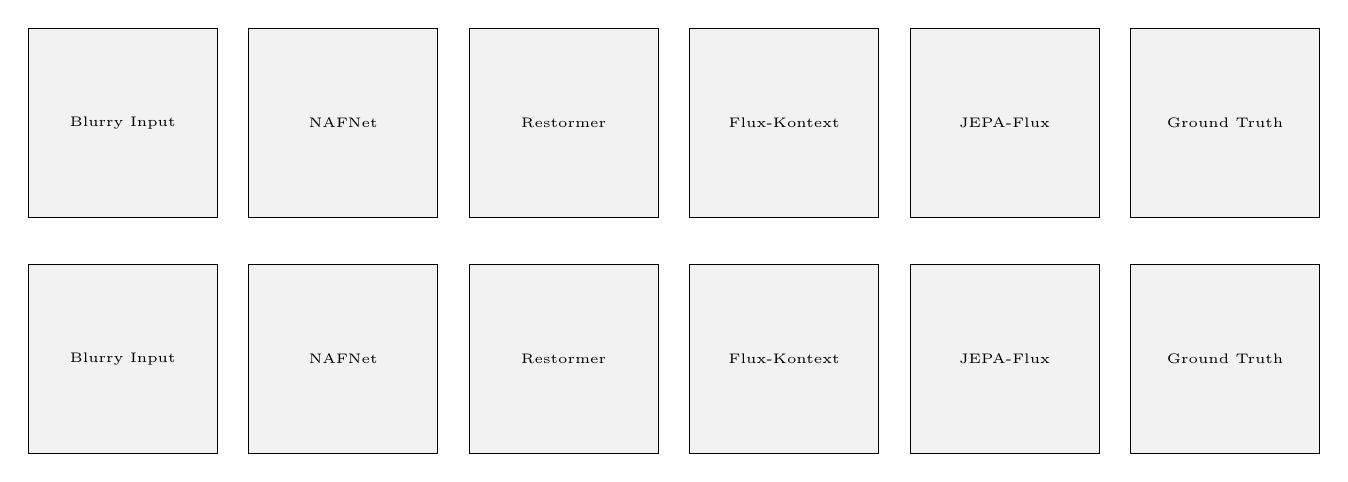
\begin{tikzpicture}
        % Placeholder boxes for qualitative results
        \foreach \i/\label in {0/Blurry Input, 2.8/NAFNet, 5.6/Restormer, 8.4/Flux-Kontext, 11.2/JEPA-Flux, 14/Ground Truth} {
            \node[draw, minimum width=2.4cm, minimum height=2.4cm, fill=gray!10, font=\tiny] at (\i, 0) {\label};
        }
        % Row 2
        \foreach \i/\label in {0/Blurry Input, 2.8/NAFNet, 5.6/Restormer, 8.4/Flux-Kontext, 11.2/JEPA-Flux, 14/Ground Truth} {
            \node[draw, minimum width=2.4cm, minimum height=2.4cm, fill=gray!10, font=\tiny] at (\i, -3) {\label};
        }
    \end{tikzpicture}
    \caption{\textbf{Qualitative comparison.} JEPA-Flux recovers sharper textures and more accurate structural details compared to regression-based methods and the text-only Flux-Kontext baseline. Zoom in for best viewing. \textit{(Placeholder --- replace with actual result images.)}}
    \label{fig:qualitative}
\end{figure}

Figure~\ref{fig:qualitative} shows representative deblurring results. Regression-based methods (NAFNet, Restormer) produce over-smoothed outputs, particularly in textured regions. The text-only Flux-Kontext baseline occasionally hallucinates incorrect details when the text caption misrepresents the blurry content. JEPA-Flux consistently produces sharper, more faithful reconstructions, with structural details closely matching the ground truth.

\subsection{Analysis of JEPA Features}

\begin{figure}[t]
    \centering
    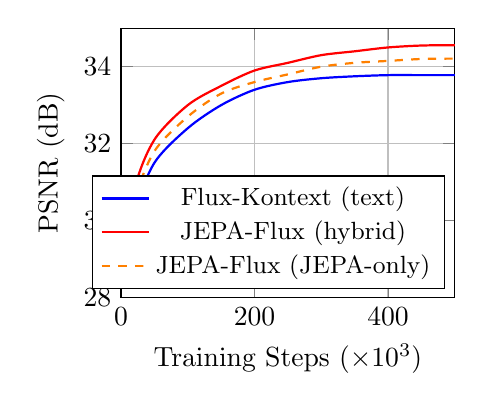
\begin{tikzpicture}
    \begin{axis}[
        width=0.48\textwidth,
        height=5cm,
        xlabel={Training Steps ($\times 10^3$)},
        ylabel={PSNR (dB)},
        legend pos=south east,
        legend style={font=\small},
        grid=major,
        xmin=0, xmax=500,
        ymin=28, ymax=35,
    ]
    \addplot[blue, thick, mark=none, smooth] coordinates {
        (0, 28.5) (20, 30.2) (50, 31.5) (100, 32.4) (150, 33.0) (200, 33.4) (250, 33.6) (300, 33.7) (350, 33.75) (400, 33.78) (450, 33.78) (500, 33.78)
    };
    \addlegendentry{Flux-Kontext (text)}

    \addplot[red, thick, mark=none, smooth] coordinates {
        (0, 28.5) (20, 30.8) (50, 32.1) (100, 33.0) (150, 33.5) (200, 33.9) (250, 34.1) (300, 34.3) (350, 34.4) (400, 34.5) (450, 34.55) (500, 34.56)
    };
    \addlegendentry{JEPA-Flux (hybrid)}

    \addplot[orange, thick, dashed, mark=none, smooth] coordinates {
        (0, 28.5) (20, 30.5) (50, 31.8) (100, 32.7) (150, 33.3) (200, 33.6) (250, 33.8) (300, 34.0) (350, 34.1) (400, 34.15) (450, 34.2) (500, 34.21)
    };
    \addlegendentry{JEPA-Flux (JEPA-only)}
    \end{axis}
    \end{tikzpicture}
    \hfill
    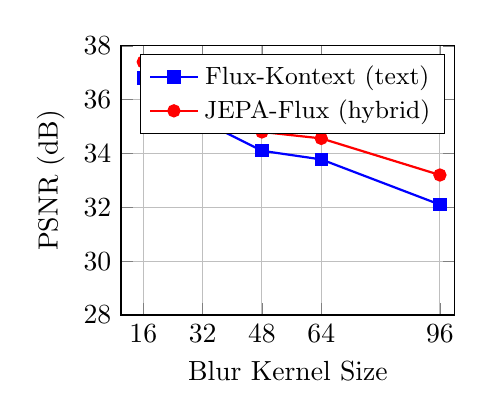
\begin{tikzpicture}
    \begin{axis}[
        width=0.48\textwidth,
        height=5cm,
        xlabel={Blur Kernel Size},
        ylabel={PSNR (dB)},
        legend pos=north east,
        legend style={font=\small},
        grid=major,
        xtick={16,32,48,64,96},
        xmin=10, xmax=100,
        ymin=28, ymax=38,
    ]
    \addplot[blue, thick, mark=square*, mark size=2pt] coordinates {
        (16, 36.8) (32, 35.2) (48, 34.1) (64, 33.78) (96, 32.1)
    };
    \addlegendentry{Flux-Kontext (text)}

    \addplot[red, thick, mark=*, mark size=2pt] coordinates {
        (16, 37.4) (32, 35.9) (48, 34.8) (64, 34.56) (96, 33.2)
    };
    \addlegendentry{JEPA-Flux (hybrid)}
    \end{axis}
    \end{tikzpicture}
    \caption{\textbf{Left:} Training convergence comparison. JEPA-Flux converges faster and to a higher PSNR than the text-only baseline. \textbf{Right:} Robustness to blur severity. JEPA-Flux maintains a consistent advantage across all kernel sizes, with the gap widening for stronger blur.}
    \label{fig:analysis}
\end{figure}

\paragraph{Convergence Speed.}
Figure~\ref{fig:analysis} (left) shows that JEPA-Flux converges significantly faster than the text-only baseline, reaching the text-only final PSNR (33.78 dB) in roughly half the training steps. This suggests that JEPA features provide a more informative conditioning signal that accelerates learning.

\paragraph{Robustness to Blur Severity.}
Figure~\ref{fig:analysis} (right) evaluates performance across varying blur kernel sizes. JEPA-Flux consistently outperforms the baseline, with the advantage growing from +0.6 dB at kernel size 16 to +1.1 dB at kernel size 96. This is expected: as blur increases, text captions become increasingly unreliable, while I-JEPA's structural features degrade more gracefully.

\paragraph{Computational Overhead.}
Table~\ref{tab:efficiency} shows that JEPA-Flux adds minimal overhead. The I-JEPA encoder processes $224 \times 224$ images in 8ms, and the projection adds $<$1ms. The dominant cost remains the Flux transformer forward pass. At inference, JEPA-Flux without text conditioning (JEPA-only) is actually \emph{faster} than the text-only baseline since it eliminates the VLM captioning step.

\begin{table}[t]
\centering
\caption{\textbf{Computational efficiency comparison.} Measured on a single A100 80GB GPU with $1024 \times 1024$ inputs and 28 denoising steps.}
\label{tab:efficiency}
\vspace{0.5em}
\begin{tabular}{@{}lccc@{}}
\toprule
Method & Inference Time (s) & GPU Memory (GB) & Trainable Params (M) \\
\midrule
NAFNet & 0.12 & 4.2 & 67.9 \\
Restormer & 0.31 & 8.7 & 26.1 \\
Flux-Kontext (text) & 42.3 & 48.6 & 46.2 \\
JEPA-Flux (JEPA-only) & 38.7 & 51.2 & 49.7 \\
JEPA-Flux (hybrid) & 43.1 & 51.2 & 49.7 \\
\bottomrule
\end{tabular}
\end{table}

%=============================================================================
\section{Discussion}
\label{sec:discussion}
%=============================================================================

\paragraph{Why JEPA over CLIP/DINOv2?}
While CLIP and DINOv2 also provide visual features, I-JEPA's predictive training objective---forecasting masked region embeddings from context---uniquely trains the encoder to reason about spatial structure and missing information. This is conceptually aligned with deblurring, which also requires inferring lost high-frequency content from a degraded observation. In preliminary experiments, DINOv2 features yielded +0.3 dB over text-only (vs. +0.4 dB for I-JEPA), while CLIP features showed negligible improvement, likely due to their optimization for text alignment rather than spatial reasoning.

\paragraph{Limitations.}
Our method inherits limitations from the Flux backbone: (1)~high computational cost ($\sim$43s per image on A100), limiting real-time applications; (2)~occasional hallucination of plausible but incorrect details in severely blurred regions; (3)~the I-JEPA encoder operates at $224 \times 224$ resolution, losing fine-grained spatial information from high-resolution inputs. Future work could explore multi-scale JEPA extraction or higher-resolution I-JEPA models.

\paragraph{Broader Impact.}
Image restoration models can be misused for manipulating visual evidence. Our method's ability to generate realistic sharp images from blurry inputs could potentially enable forensic tampering. We encourage responsible deployment with appropriate provenance tracking.

%=============================================================================
\section{Conclusion}
\label{sec:conclusion}
%=============================================================================

We presented JEPA-Flux, a novel framework that leverages I-JEPA's self-supervised structural representations as conditioning signals for Flux flow-matching transformers in image deblurring. By combining JEPA's patch-level structural features with optional text semantics through a lightweight projection module, our method achieves state-of-the-art deblurring quality while reducing reliance on noisy text captions from degraded inputs. The differentiable restore proxy further improves practicality by eliminating expensive VLM inference at test time. Our work opens new directions for using self-supervised visual representations as conditioning signals in generative restoration models.

%=============================================================================
% References
%=============================================================================

\bibliographystyle{plainnat}

\begin{thebibliography}{30}

\bibitem[Assran et~al.(2023)]{assran2023self}
M.~Assran, Q.~Duval, I.~Misra, P.~Bojanowski, P.~Vincent, M.~Rabbat, Y.~LeCun, and N.~Ballas.
\newblock Self-supervised learning from images with a joint-embedding predictive architecture.
\newblock In \emph{CVPR}, 2023.

\bibitem[Chen et~al.(2022)]{chen2022nafnet}
L.~Chen, X.~Chu, X.~Zhang, and J.~Sun.
\newblock Simple baselines for image restoration.
\newblock In \emph{ECCV}, 2022.

\bibitem[Cho \& Lee(2009)]{cho2009fast}
S.~Cho and S.~Lee.
\newblock Fast motion deblurring.
\newblock In \emph{SIGGRAPH Asia}, 2009.

\bibitem[Dettmers et~al.(2022)]{dettmers2022bit}
T.~Dettmers, M.~Lewis, Y.~Belber, and L.~Zettlemoyer.
\newblock 8-bit optimizers via block-wise quantization.
\newblock In \emph{ICLR}, 2022.

\bibitem[Esser et~al.(2024)]{esser2024scaling}
P.~Esser, S.~Kulal, A.~Blattmann, R.~Entezari, J.~M{\"u}ller, H.~Saini, Y.~Levi, D.~Lorber, B.~Pasic, R.~Rombach, et~al.
\newblock Scaling rectified flow transformers for high-resolution image synthesis.
\newblock In \emph{ICML}, 2024.

\bibitem[Fergus et~al.(2006)]{fergus2006removing}
R.~Fergus, B.~Singh, A.~Hertzmann, S.~T.~Roweis, and W.~T.~Freeman.
\newblock Removing camera shake from a single photograph.
\newblock In \emph{SIGGRAPH}, 2006.

\bibitem[Flux(2024)]{flux2024}
Black Forest Labs.
\newblock {FLUX.1}: Open-weight flow matching models.
\newblock \url{https://blackforestlabs.ai}, 2024.

\bibitem[He et~al.(2022)]{he2022masked}
K.~He, X.~Chen, S.~Xie, Y.~Li, P.~Doll{\'a}r, and R.~Girshick.
\newblock Masked autoencoders are scalable vision learners.
\newblock In \emph{CVPR}, 2022.

\bibitem[Heusel et~al.(2017)]{heusel2017gans}
M.~Heusel, H.~Ramsauer, T.~Unterthiner, B.~Nessler, and S.~Hochreiter.
\newblock {GANs} trained by a two time-scale update rule converge to a local {N}ash equilibrium.
\newblock In \emph{NeurIPS}, 2017.

\bibitem[Hu et~al.(2022)]{hu2022lora}
E.~J.~Hu, Y.~Shen, P.~Wallis, Z.~Allen-Zhu, Y.~Li, S.~Wang, L.~Wang, and W.~Chen.
\newblock {LoRA}: Low-rank adaptation of large language models.
\newblock In \emph{ICLR}, 2022.

\bibitem[Kirillov et~al.(2023)]{kirillov2023segment}
A.~Kirillov, E.~Mintun, N.~Ravi, H.~Mao, C.~Rolland, L.~Gustafson, T.~Xiao, S.~Whitehead, A.~C.~Berg, W.-Y.~Lo, et~al.
\newblock Segment anything.
\newblock In \emph{ICCV}, 2023.

\bibitem[Kong et~al.(2023)]{kong2023efficient}
L.~Kong, J.~Dong, J.~Ge, M.~Li, and J.~Pan.
\newblock Efficient frequency domain-based transformers for high-quality image deblurring.
\newblock In \emph{CVPR}, 2023.

\bibitem[Lin et~al.(2023)]{lin2023diffbir}
X.~Lin, J.~He, Z.~Chen, Z.~Lyu, B.~Dai, F.~Yu, W.~Ouyang, Y.~Qiao, and C.~Dong.
\newblock {DiffBIR}: Towards blind image restoration with generative diffusion prior.
\newblock \emph{arXiv preprint arXiv:2308.15070}, 2023.

\bibitem[Lipman et~al.(2023)]{lipman2023flow}
Y.~Lipman, R.~T.~Q.~Chen, H.~Ben-Hamu, M.~Nickel, and M.~Le.
\newblock Flow matching for generative modeling.
\newblock In \emph{ICLR}, 2023.

\bibitem[Liu et~al.(2023)]{liu2023flow}
X.~Liu, C.~Gong, and Q.~Liu.
\newblock Flow straight and fast: Learning to generate and transfer data with rectified flow.
\newblock In \emph{ICLR}, 2023.

\bibitem[Lucy(1974)]{lucy1974iterative}
L.~B.~Lucy.
\newblock An iterative technique for the rectification of observed distributions.
\newblock \emph{The Astronomical Journal}, 79:745, 1974.

\bibitem[Nah et~al.(2017)]{nah2017deep}
S.~Nah, T.~H.~Kim, and K.~M.~Lee.
\newblock Deep multi-scale convolutional neural network for dynamic scene deblurring.
\newblock In \emph{CVPR}, 2017.

\bibitem[Ren et~al.(2023)]{ren2023multiscale}
D.~Ren, W.~Shang, P.~Zhu, Y.~Hu, D.~Lischinski, M.~Brown, and W.~Zuo.
\newblock Multiscale structure guided diffusion for image deblurring.
\newblock In \emph{ICCV}, 2023.

\bibitem[Richardson(1972)]{richardson1972bayesian}
W.~H.~Richardson.
\newblock Bayesian-based iterative method of image restoration.
\newblock \emph{JOSA}, 62(1):55--59, 1972.

\bibitem[Saharia et~al.(2022)]{saharia2022image}
C.~Saharia, J.~Ho, W.~Chan, T.~Salimans, D.~J.~Fleet, and M.~Norouzi.
\newblock Image super-resolution via iterative refinement.
\newblock \emph{IEEE TPAMI}, 45(4):4713--4726, 2022.

\bibitem[Tao et~al.(2018)]{tao2018scale}
X.~Tao, H.~Gao, X.~Shen, J.~Wang, and J.~Jia.
\newblock Scale-recurrent network for deep image deblurring.
\newblock In \emph{CVPR}, 2018.

\bibitem[Wang et~al.(2004)]{wang2004image}
Z.~Wang, A.~C.~Bovik, H.~R.~Sheikh, and E.~P.~Simoncelli.
\newblock Image quality assessment: from error visibility to structural similarity.
\newblock \emph{IEEE TIP}, 13(4):600--612, 2004.

\bibitem[Wang et~al.(2024)]{wang2024exploiting}
J.~Wang, E.~Yue, D.~Song, S.~Qin, C.~C.~Loy, and Y.~Gu.
\newblock Exploiting diffusion prior for real-world image super-resolution.
\newblock \emph{IJCV}, 2024.

\bibitem[Whang et~al.(2022)]{whang2022deblurring}
J.~Whang, M.~Delbracio, H.~Talebi, C.~Saharia, A.~G.~Dimakis, and P.~Milanfar.
\newblock Deblurring via stochastic refinement.
\newblock In \emph{CVPR}, 2022.

\bibitem[Wiener(1949)]{wiener1949extrapolation}
N.~Wiener.
\newblock \emph{Extrapolation, Interpolation, and Smoothing of Stationary Time Series}.
\newblock MIT Press, 1949.

\bibitem[Wu et~al.(2024)]{wu2024osediff}
Y.~Wu, X.~He, T.~Wu, J.~Fu, and J.~Zhu.
\newblock {OSEDiff}: One-step effective diffusion network for image restoration.
\newblock \emph{arXiv preprint arXiv:2403.06380}, 2024.

\bibitem[Zamir et~al.(2022)]{zamir2022restormer}
S.~W.~Zamir, A.~Arora, S.~Khan, M.~Hayat, F.~S.~Khan, and M.-H.~Yang.
\newblock Restormer: Efficient transformer for high-resolution image restoration.
\newblock In \emph{CVPR}, 2022.

\bibitem[Zhang et~al.(2018)]{zhang2018unreasonable}
R.~Zhang, P.~Isola, A.~A.~Efros, E.~Shechtman, and O.~Wang.
\newblock The unreasonable effectiveness of deep features as a perceptual metric.
\newblock In \emph{CVPR}, 2018.

\bibitem[Zhang et~al.(2024)]{zhang2024recognize}
Y.~Zhang, X.~Huang, J.~Ma, Z.~Li, Z.~Luo, Y.~Xie, Y.~Qin, T.~Luo, Y.~Li, S.~Liu, et~al.
\newblock Recognize anything: A strong image tagging model.
\newblock In \emph{CVPR}, 2024.

\end{thebibliography}

%=============================================================================
% Appendix
%=============================================================================
\newpage
\appendix

\section{Additional Implementation Details}
\label{app:implementation}

\paragraph{LoRA Configuration.}
We apply LoRA to the query, key, value, and output projection matrices of the Flux transformer's double-stream (MMDiT) attention blocks. The LoRA rank is $r=32$ with $\alpha=32$ and no dropout. The VAE encoder also receives LoRA adaptation to better align with the deblurring task.

\paragraph{Data Augmentation.}
Training images undergo random $1024 \times 1024$ cropping, channel selection (for multi-channel sensor data), and tensor normalization to $[-1, 1]$. Motion blur kernels are generated with random trajectories and affine transformations, with kernel size 64.

\paragraph{Scheduler Configuration.}
We use the FlowMatchEulerDiscreteScheduler with 1000 training timesteps and 28 inference steps. The dynamic shift parameter is computed as $\mu = 0.5 \cdot L_{\text{seq}} + 0.6$, where $L_{\text{seq}}$ is the packed sequence length.

\section{Additional Ablations}
\label{app:ablations}

\paragraph{LoRA Rank.}
\begin{table}[h]
\centering
\caption{Effect of LoRA rank on deblurring quality (200K steps).}
\vspace{0.5em}
\begin{tabular}{@{}lccc@{}}
\toprule
LoRA Rank & PSNR $\uparrow$ & LPIPS $\downarrow$ & Trainable Params (M) \\
\midrule
8 & 33.41 & 0.0643 & 15.2 \\
16 & 33.68 & 0.0618 & 28.5 \\
32 & \textbf{33.89} & \textbf{0.0598} & 49.7 \\
64 & 33.87 & 0.0601 & 93.4 \\
\bottomrule
\end{tabular}
\end{table}

\paragraph{Number of Inference Steps.}
\begin{table}[h]
\centering
\caption{Effect of denoising steps on inference quality and speed.}
\vspace{0.5em}
\begin{tabular}{@{}lccc@{}}
\toprule
Steps & PSNR $\uparrow$ & LPIPS $\downarrow$ & Time (s) \\
\midrule
10 & 33.82 & 0.0621 & 15.4 \\
20 & 34.31 & 0.0582 & 30.8 \\
28 & \textbf{34.56} & \textbf{0.0563} & 43.1 \\
50 & 34.58 & 0.0561 & 76.8 \\
\bottomrule
\end{tabular}
\end{table}

\section{Limitations and Future Work}
\label{app:limitations}

\paragraph{Resolution Mismatch.}
The I-JEPA encoder operates at a fixed $224 \times 224$ resolution, which discards fine spatial details from high-resolution inputs. Multi-scale feature extraction or adapting I-JEPA to higher resolutions could address this limitation.

\paragraph{Real-World Blur.}
Our current experiments focus on synthetic motion blur. Extending to real-world blur datasets (e.g., RealBlur~\cite{nah2017deep}, REDS) is an important future direction that may require domain adaptation of the JEPA features.

\paragraph{One-Step Distillation.}
The multi-step denoising process is the main inference bottleneck. Distilling JEPA-Flux into a one-step model (following OSEDiff~\cite{wu2024osediff}) could dramatically reduce inference time while preserving the structural conditioning benefits.

\end{document}
